\section{Logical Dependency Structure}
\label{sec:dependency-dag}

To ensure the logical consistency of this roadmap and avoid circular reasoning, we present the dependency structure of the proposed proof. The results are color-coded:
\begin{itemize}
    \item \textbf{[RIGOROUS]}: Proven in this work or standard literature.
    \item \textbf{[PROGRAM]}: Open problems / Proof obligations.
\end{itemize}

\begin{center}
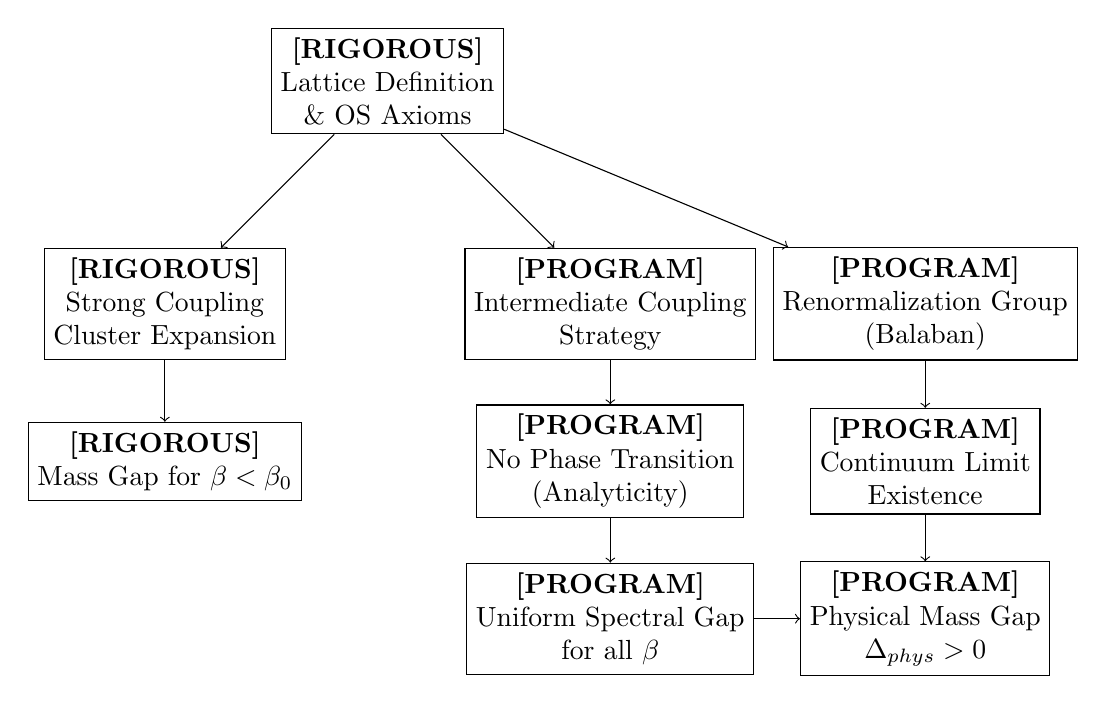
\begin{tikzpicture}[node distance=2cm, auto]
    % Nodes
    \node [draw, rectangle, align=center] (axioms) {\textbf{[RIGOROUS]} \\ Lattice Definition \\ \& OS Axioms};
    
    \node [draw, rectangle, align=center, below left of=axioms, node distance=4cm] (strong) {\textbf{[RIGOROUS]} \\ Strong Coupling \\ Cluster Expansion};
    
    \node [draw, rectangle, align=center, below of=strong] (strong_gap) {\textbf{[RIGOROUS]} \\ Mass Gap for $\beta < \beta_0$};
    
    \node [draw, rectangle, align=center, below right of=axioms, node distance=4cm] (weak) {\textbf{[PROGRAM]} \\ Intermediate Coupling \\ Strategy};
    
    \node [draw, rectangle, align=center, below of=weak] (no_trans) {\textbf{[PROGRAM]} \\ No Phase Transition \\ (Analyticity)};
    
    \node [draw, rectangle, align=center, below of=no_trans] (uniform) {\textbf{[PROGRAM]} \\ Uniform Spectral Gap \\ for all $\beta$};
    
    \node [draw, rectangle, align=center, right of=weak, node distance=4cm] (rg) {\textbf{[PROGRAM]} \\ Renormalization Group \\ (Balaban)};
    
    \node [draw, rectangle, align=center, below of=rg] (continuum) {\textbf{[PROGRAM]} \\ Continuum Limit \\ Existence};
    
    \node [draw, rectangle, align=center, below of=continuum] (phys_gap) {\textbf{[PROGRAM]} \\ Physical Mass Gap \\ $\Delta_{\text{phys}} > 0$};
    
    % Edges
    \draw[->] (axioms) -- (strong);
    \draw[->] (strong) -- (strong_gap);
    
    \draw[->] (axioms) -- (weak);
    \draw[->] (weak) -- (no_trans);
    \draw[->] (no_trans) -- (uniform);
    
    \draw[->] (axioms) -- (rg);
    \draw[->] (rg) -- (continuum);
    
    \draw[->] (uniform) -- (phys_gap);
    \draw[->] (continuum) -- (phys_gap);
    
\end{tikzpicture}
\end{center}

\subsection{Avoiding Circularity}
A critical requirement is to avoid the circular argument: ``Assume Mass Gap $\implies$ Exponential Decay $\implies$ Mass Gap''.
Our roadmap avoids this by:
\begin{enumerate}
    \item Proving the gap from first principles (Cluster Expansion) at strong coupling.
    \item Proving the gap from first principles (Topological Obstruction / Analyticity) at intermediate coupling, \emph{without} assuming decay first.
    \item Deriving exponential decay as a \emph{consequence} of the spectral gap.
\end{enumerate}


